\documentclass[preprint,12pt,ntfdMod]{elsarticle}
\usepackage{graphicx}
\usepackage{color}
\usepackage[numbered,bw]{mcode}
\usepackage{amsmath}
\usepackage{amsfonts}
\usepackage{natbib}
\usepackage{hyperref}
\usepackage{esint}
\usepackage{subfig}
\usepackage[subfigure]{tocloft}
\usepackage{units}
\usepackage[protrusion=true,expansion]{microtype}
\hypersetup{
	bookmarks=true,         % show bookmarks bar?
	unicode=false,          % non-Latin characters in Acrobat’s bookmarks
	pdftoolbar=true,        % show Acrobat’s toolbar?
	pdfmenubar=true,        % show Acrobat’s menu?
	pdffitwindow=false,     % window fit to page when opened
	pdfstartview={FitH},    % fits the width of the page to the window
	pdftitle={My title},    % title
	pdfauthor={Author},     % author
	pdfsubject={Subject},   % subject of the document
	pdfcreator={Creator},   % creator of the document
	pdfproducer={Producer}, % producer of the document
	pdfkeywords={keyword1} {key2} {key3}, % list of keywords
	pdfnewwindow=true,      % links in new window
	colorlinks=true,       % false: boxed links; true: colored links
	linkcolor=red,          % color of internal links
	citecolor=green,        % color of links to bibliography
	filecolor=magenta,      % color of file links
	urlcolor=cyan           % color of external links
}
\usepackage{verbatim}
\usepackage{relsize}
\usepackage{lipsum}
\usepackage{caption}
\captionsetup[figure]{name=Fig.,labelfont=bf}
\setlength{\cftbeforesecskip}{2pt}

\definecolor{lightgray}{gray}{0.5}
\setlength{\parindent}{0pt}

%c from texinfo.tex
\def\ifmonospace{\ifdim\fontdimen3\font=0pt }
%c C plus plus
\def\C++{%
\ifmonospace%
    C++%
	\else%
	    C\kern-.1667em\raise.30ex\hbox{\smaller{++}}%
		\fi%
		\spacefactor1000 }
\lstset{%
xleftmargin=8mm,%
xrightmargin=8mm,%
framexleftmargin=6mm,%
xleftmargin=6mm,%
breaklines=true}

\author[rss]{Felix Dietzsch}
\address[rss]{Institut f\"ur Chemieingenieurwesen und Energieverfahrenstechnik,...}
\title{Small post processor}
\begin{document}
		\maketitle 
		\tableofcontents

\section{Clear complete workspace}

\begin{par}
For new Matlab projects best practise is to clear the complete workspace and the command window. It is also a good habit to close all remaining figures since Matlab does not automatically open a new window each time a plot call is invoked.
\end{par} \vspace{1em}
\begin{verbatim}
display('Clear workspace ...')
path('./functions',path) % add functions directory the Matlab path
close all % close all figures
clear all % clear workspace
clc % clear command window
%set(0,'DefaultFigureWindowStyle','docked')
[datadir,flag]=ClearWs();
\end{verbatim}

        \color{lightgray} \begin{verbatim}Clear workspace ...
\end{verbatim} \color{black}
    \begin{par}

The above mentioned clears are performed in the function \verb|ClearWs|.
In addition some basic parameters like the name of the data
directory or the dimensionality of the problem are also defined.
\lstinputlisting{../functions/ClearWs.m}

\end{par} \vspace{1em}


\section{Read data files}

\begin{par}

During the evaluation of the function \verb|ReadData| all data files
neseccary for the calculation of the spectrum and the correlation
coefficients are read, namely the velocity components. In addition the
import operations are enclosed in a \lstinline!tic;!$\ldots$
\lstinline!;toc! block
measuring the time needed for reading the ASCII data. What you should
get from the tic/toc
block is that most of the time is spend during data I/O
(Input/Output operations), nearly \unit[220]{s}. The actual computation
needs only about \unit[8]{s}. What you can easily calculate from this is
that the
computation of the spectrum is nearly 27 times faster then the data
import. Why the computation of Fourier transforms is that fast we will
come to that later.
Although the ASCII
data format ist not the prefered choice in terms of speed and size, we
will use it since other
methodologies require additional knowledge of data processing. Just for
your information a very famous and highly protable data format is
\href{http://www.hdfgroup.org/HDF5/}{hdf5}. It is a software library that
runs on a range of computational platforms, from laptops to massively
parallel systems and implements a high-level API (Application
programming interface) with C, \C++, Fortran 90,
and Java interfaces. Besides its hierarchical
structure it is highly optimized for parallel I/O operations and can be
read by nearly all data processing tools.

\end{par} \vspace{1em}
\begin{verbatim}
display('Read data ...')
[uvel,vvel,wvel,time_read] = ReadData(datadir,flag,'uvel','vvel','wvel');
% test=importdata('data/3D/CFX_velocity_field.dat');
% uvel=reshape(test(:,1),33,33,33);
% vvel=reshape(test(:,2),33,33,33);
% wvel=reshape(test(:,3),33,33,33);
\end{verbatim}

        \color{lightgray} \begin{verbatim}Read data ...
\end{verbatim} \color{black}
    \begin{par}

\lstinputlisting{../functions/ReadData.m}

\end{par} \vspace{1em}


\section{Set neccessary parameters}

\begin{par}

For further computations it is important to define some parmeters of the
DNS simulation such as
\begin{itemize}
  \item Number of grid points in on direction $n_{p}$,
  \item Physical length of one direction $L_x$,
  \item Physical grid spacing $\triangle x$,
  \item Kinematic viscosity $\nu$.
\end{itemize}

\end{par} \vspace{1em}
\begin{verbatim}
display('Set parameters ...')
[u,v,w,dim,Lx,dx,nu]=Params(uvel,vvel,wvel);
% u=u-mean2(u);
% v=v-mean2(v);
% w=w-mean2(w);
\end{verbatim}

        \color{lightgray} \begin{verbatim}Set parameters ...
\end{verbatim} \color{black}
    \begin{par}

\lstinputlisting{../functions/Params.m}

\end{par} \vspace{1em}


\section{Compute 3D spectrum}

\begin{par}

The core of the code is contained in the function
\lstinline!PowerSpec!. It computes the three dimensional energy spectrum
from the given velocity fields, obtained from a direct numerical
simulation. Although the theoretical analysis is
relatively demanding compared to one dimensional spectra its worth
investing the effort.
The theory of one dimensional spectra relies
on the assumption that the propagation of spectral waves ($\kappa_1$)
is in the direction of the observed velocity fields or to say it differently one
dimenional spectra and correlation functions are Fourier transform pairs.
The theory of correlation functions will be discussed in section \ref{sec:correlation}.
A key drawback of this theory is that the calculated spectrum has
contributions from all wavenumbers $\boldsymbol\kappa$, so that the
magnitude of $\boldsymbol\kappa$ can be appreciably larger than
$\kappa_1$. This phenomenon is called aliasing.
In order to avoid these aliasing effects is also possible to produce correlations that
involve all possible directions. The three dimensional Fourier
transformation of such a correlation produces a spectrum that not only
depends on a single wavenumber but on the wavenumber vector $\kappa_i$.
Though the directional information contained in $\kappa_i$ eliminates the
aliasing problem the complexity makes a physical reasoning impossible.
For homogeneous isotropic turbulence the situation can be considerably
simplified. From the knowledge that the velocity field is isotropic it can be
shown that the velocity spectrum tensor is fully determined by
  \begin{equation}
      \label{eq:iso_tensor}
      \Phi_{ij}(\boldsymbol\kappa) = A(\kappa)\delta_{ij}+B(\kappa)\kappa_i\kappa_j,
  \end{equation}
where $A(\kappa)$ and $B(\kappa)$ are arbitrary scalar functions. Since we assume
incompressible fluids (mathematically expressed by $\nabla\cdot u=0$ or $\kappa_iu_i=0$
the following condition holds
  \begin{equation}
      \kappa_i\,\Phi_{ij}(\boldsymbol\kappa)=0.
  \end{equation}
It can be shown that this yields a relation between $A$ and $B$ by means of
  \begin{equation}
      \label{eq:rel_AB}
  	B(\kappa)=-\frac{A(\kappa)}{\kappa^2}
  \end{equation}
In the end this gives a relation between the three dimensional energy spectrum
function $E(|\boldsymbol\kappa|)$ and the velocity spectrum tensor $\Phi_{ij}$.
  \begin{equation}
  	\Phi_{ij}=\frac{E(|\boldsymbol\kappa|)}{4\pi\,(|\boldsymbol\kappa|)^2}\left(\delta_{ij}
  	-\frac{\kappa_i\kappa_j}{(|\boldsymbol\kappa|)^2}\right)
  \end{equation}
The question is now how the remaining variable ($A$ or $B$) can be determined. Regarding the turbulent kinetic
energy we know that
  \begin{equation}
      \label{eq:exp_for_k}
      k=\int\limits_{-\infty}^{\infty}E(|\boldsymbol\kappa|)\,\mathrm{d}k
      =\sum\limits_{\boldsymbol\kappa}E(\boldsymbol\kappa)
      =\sum\limits_{\boldsymbol\kappa}\frac{1}{2}\left<u^{*}(\boldsymbol\kappa)\,u(\boldsymbol\kappa)\right>
      =\iiint\limits_{-\infty}^{\infty}\frac{1}{2}\Phi_{ii}(\boldsymbol\kappa)\,\mathrm{d}\boldsymbol\kappa.
  \end{equation}
Comparing the second and last expression we get
  \begin{equation}
      E(|\boldsymbol\kappa|)=\oiint\frac{1}{2}\,\Phi_{ii}(\boldsymbol\kappa)\,\mathrm{d}S(\kappa).
  \end{equation}
  \begin{figure}[t!]
      \centering
      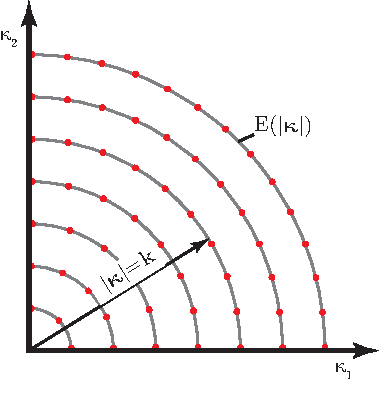
\includegraphics[scale=1]{shell_integration}
      \caption{Illustration of the two dimensional shell integration}
      \label{fig:shell_int}
  \end{figure}
This integral can be solved analytically by utilizing again the assumption of isotropy.
For these kind of flows the energy spectrum function can be regarded as the sum of kinetic energy
(in wave number space) on different energy levels. Each of these energy levels is denoted by a spherical
shell in wave number space. Since the surface of a sphere is completly determined by its radius the
surface integral can be solved analytically. The idea of this integration is illustrated
in Fig. \ref{fig:shell_int}.
As a result of this one gets
  \begin{equation}
      E(|\boldsymbol\kappa|)=\oiint\frac{1}{2}\,\Phi_{ii}(\boldsymbol\kappa)\,\mathrm{d}S(\kappa)
      =4\pi(|\boldsymbol\kappa|)^2\,\Phi_{ii}(|\boldsymbol\kappa|).
  \end{equation}
Introducing this relation to equations \eqref{eq:iso_tensor} and
\eqref{eq:rel_AB} one arrives at an expression for the variable $B$.
  \begin{equation}
      B=-\frac{E(|\boldsymbol\kappa|)}{4\pi(|\boldsymbol\kappa|)^2}
  \end{equation}
Together with the approximation of the integral of $\Phi$
(equation \eqref{eq:exp_for_k})
  \begin{equation}
      \iiint\limits_{-\infty}^{\infty}\frac{1}{2}\Phi_{ii}(\boldsymbol\kappa)\,\mathrm{d}\boldsymbol\kappa
      \approx\frac{1}{2}\sum\limits_{\boldsymbol\kappa}\Phi_{ii}(\boldsymbol\kappa)\,(\Delta\kappa)^3,
  \end{equation}
where $\Delta\kappa$ refers to the step size in wave number space,
the final expression of the three dimensional discrete energy spectrum can be derived.
  \begin{equation}
      E(|\boldsymbol\kappa|)=2\pi(|\boldsymbol\kappa|)^2\frac{\left<u^{*}
      (\boldsymbol\kappa)\,u(\boldsymbol\kappa)\right>}{(\Delta\kappa)^3}
  \end{equation}
The calling sequence for the computation of the energy spectrum reads
  \begin{figure}[t!]
      \centering
      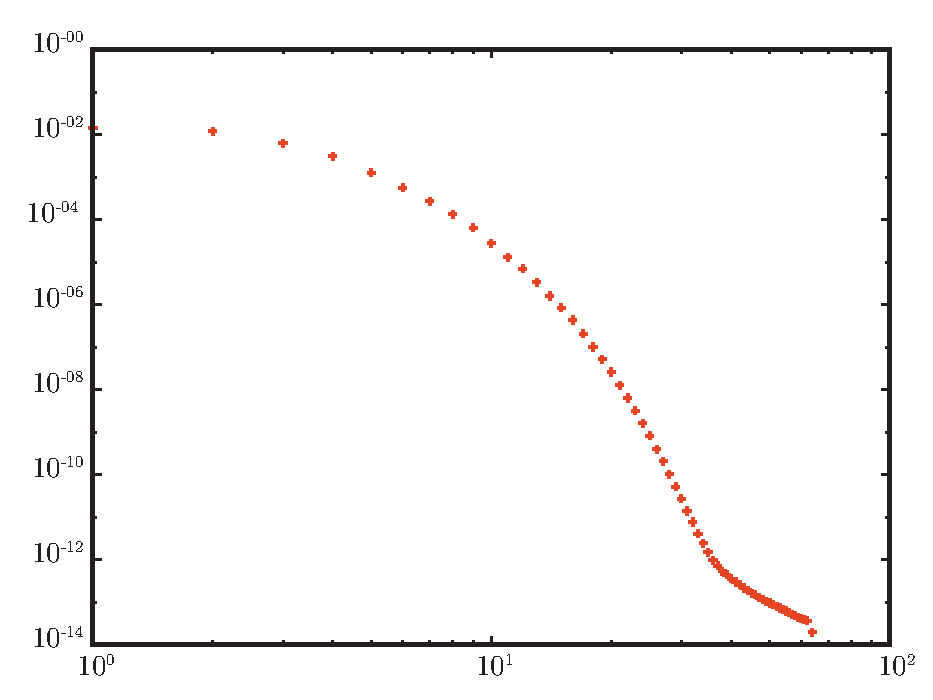
\includegraphics[scale=1]{spectrum}
	  \caption{Power spectrum}
      \label{fig:spectrum}
  \end{figure}

\end{par} \vspace{1em}
\begin{verbatim}
display('Compute spectrum...')
[spectrum,k,bin_counter,time_spec] = PowerSpec(u,v,w,Lx,dim);
\end{verbatim}

        \color{lightgray} \begin{verbatim}Compute spectrum...
\end{verbatim} \color{black}
    \begin{par}

\lstinputlisting{../functions/PowerSpec.m}

\end{par} \vspace{1em}


\section{Compute dissipation and turbulent kinetic energy}

\begin{par}

  The function \lstinline!SpecProp! calculates the kinetic energy both
  from the velocities and the previously computed spectrum. The latter
  one is calcualted by
  \begin{equation}
      k = \int\limits_{-\infty}^{\infty} E(|\boldsymbol\kappa|)\,\mathrm{d}|\boldsymbol\kappa|
  \end{equation}
  A second integral, also evaluated in this routine, gives the value
  of the Dissipation
  \begin{equation}
      \epsilon = 2\int\limits_{-\infty}^{\infty}\nu(|\boldsymbol\kappa|)^2
      E(|\boldsymbol\kappa|)\,\mathrm{d}|\boldsymbol\kappa|,
  \end{equation}
  where $\nu$ refers to the kinematic viscosity.
  The calling sequence reads

\end{par} \vspace{1em}
\begin{verbatim}
display('Compute kinetic energy...')
[Dissipation,kin_E_Sp,kin_E_Ph,up] = SpecProp(spectrum,k,...
                                            nu,u,v,w,dim);
\end{verbatim}

        \color{lightgray} \begin{verbatim}Compute kinetic energy...
\end{verbatim} \color{black}
    \begin{par}

\lstinputlisting{../functions/SpecProp.m}

\end{par} \vspace{1em}


\section{Kolmogorov properties}

\begin{par}

According to the Kolomogorov hypotheses the length scale $\eta$,
characterisitc velocity $u_{\eta}$ and the characteristic time scale
$\tau$ of the smallest swirls in the flow are computed
within the function \lstinline!KolmoScale!. From a dimensionality
analysis Kolmogorov derived
  \begin{eqnarray}
      \eta&=\displaystyle\left(\frac{\nu^3}{\epsilon}\right)^{1/4},\\
      u_{\eta}&=\left(\epsilon\,\nu\right)^{1/4},\\
      \tau_{\eta}&=\displaystyle\left(\frac{\nu}{\epsilon}\right)^{1/2}.
  \end{eqnarray}
For further reading concerning his theory it is refered to
\citet{Pope:2000tp}, \citet{Hinze:1975tb} and \citet{Tennekes:1972vb}.

\end{par} \vspace{1em}
\begin{verbatim}
display('Compute Kolmogorov scales...')
[eta,u_eta,tau]=KolmoScale(nu,Dissipation);
\end{verbatim}

        \color{lightgray} \begin{verbatim}Compute Kolmogorov scales...
\end{verbatim} \color{black}
    \begin{par}

\lstinputlisting{../functions/KolmoScale.m}

\end{par} \vspace{1em}


\section{Compute correlations}

\begin{par}

\label{sec:correlation}
From a general perspective correlation functions are a measure of how
much two physical quantities are connected. So how is this helpful for
the analysis of turbulent flows? For seemingly chaotic and random
procescees it would be beneficial if we had a measure of how the velocity
at point $A$ is influenced by the velocity at point $B$. A maybe more
intuitive quantity that can be calculated from the correlation functions
is the integral lengthscale which gives a measure of the largest
eddies in the flow. In fluid dynamics one generally differentiates
between two forms of correlation functions, the longitudinal and the
transversal or lateral correlation function. The difference between both forms is
illustrated in figure \ref{fig:correlations}.
\begin{figure}[t!]
        \centering
        \subfloat[Longitudinal correlation][Longitudinal correlation]{
        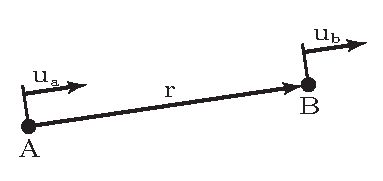
\includegraphics[scale=1]{long_corr.eps}
        \label{fig:long_corr}
        }
        \hfill
        \subfloat[Transversal correlation][Transversal correlation]{
        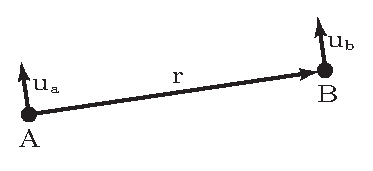
\includegraphics[scale=1]{trans_corr.eps}
        \label{fig:trans_corr}
        }
\caption{Illustration of different correlation functions}
\label{fig:correlations}
\end{figure}
In general the correlation between two components of an isotropic
homogeneous velocity field is expressed by
  \begin{equation}
      R_{ij} = \left<u_i(\mathbf{x}+r)\,u_j(\mathbf{x})\right>.
  \end{equation}
The correlation coefficients are computed by normalizing
$R_{ij}$ with the square root of the product of the two variances
$\sigma_i^2$ and $\sigma_j^2$.
  \begin{equation}
      r_{ij} = \frac{\left<u_i(\mathbf{x}+\mathbf{r})\,u_j(\mathbf{x})\right>}
                  {\sqrt{\sigma_i^2\,\sigma_j^2}}
  \end{equation}
As illustrated in figure \ref{fig:correlations} the longitudinal and lateral
correlation depend on the direction of $\mathbf{r}$, i.e.
  \begin{eqnarray}
      f(r) &= \displaystyle\frac{\left<u_1(\mathbf{x}+r\mathbf{e}_1)\,u_1(\mathbf{x})\right>}
                  {\sigma_1}\\
      g(r) &= \displaystyle\frac{\left<u_2(\mathbf{x}+r\mathbf{e}_1)\,u_2(\mathbf{x})\right>}
                  {\sigma_2}
  \end{eqnarray}
From several theoretical analysis it is well known that correlations can
be efficiently computed by means of multiplying the Fourier transform of
a quantity with its complex conjugate. Using the FFT approach this gives
an enormeous speed advantage.
  \begin{equation}
      R_{ij} =
      \mathfrak{F}^{-1}\left\{\mathfrak{F}\left\{u_i\right\}^*\cdot\mathfrak{F}\left\{u_j\right\}\right\}
  \end{equation}

\end{par} \vspace{1em}
\begin{verbatim}
display('Compute Correlations...')
[R11,R22,r,R1,R2,R3]=Correlation(u,v,w,Lx,dim);
\end{verbatim}

        \color{lightgray} \begin{verbatim}Compute Correlations...
Warning: Integer operands are required for colon operator when used as
index 
Warning: Integer operands are required for colon operator when used as
index 
\end{verbatim} \color{black}
    \begin{par}

The content of \verb|Correlation| reads
\lstinputlisting{../functions/Correlation.m}

\end{par} \vspace{1em}
\begin{par}

\bibliographystyle{NTFD-bibstyle}
\bibliography{bibliography}

\end{par} \vspace{1em}


\section{Plotting}

\begin{verbatim}
display('Save results...')
close all
h = figure('visible','on')
comte=importdata('Comte-Bellot.txt');
kC=comte.data(:,1).*100;
EC=comte.data(:,2)./100^3;
vkp=importdata('data/3D/CTRL_TURB_ENERGY');
h=loglog(vkp(:,1),vkp(:,3),'*-b');hold on
set(h,'LineWidth',1);
h=loglog(k,spectrum,'r-s');
set(h,'LineWidth',1);
h=loglog(kC,EC,'*-g');
set(h,'LineWidth',1);
legend('VKP','Dietzsch','Comte-Bellot')
saveas(gcf,'spectrum.eps','psc2')
\end{verbatim}

        \color{lightgray} \begin{verbatim}Save results...

h =

     1

\end{verbatim} \color{black}
    
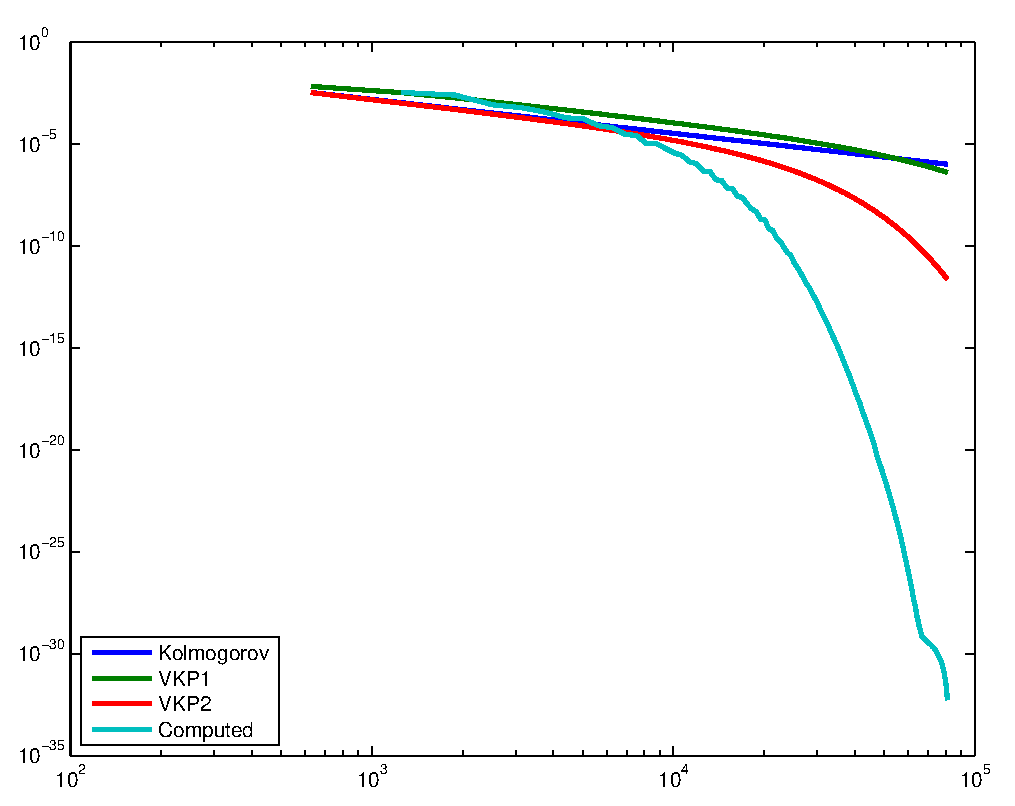
\includegraphics [width=4in]{spectrum_3d_01.eps}



\end{document}
    
